\documentclass[14pt]{extarticle}
\usepackage{amsmath,amsthm,amssymb}
\usepackage{mathtext}

\usepackage[a4paper, top=2cm, bottom=2cm, left=3cm, right=1cm]{geometry}

\usepackage[T1,T2A]{fontenc}
\usepackage[utf8]{inputenc}
\usepackage[english,russian]{babel}

\usepackage{epsfig}

\usepackage{verbatim}

\usepackage{setspace}
\onehalfspacing

\usepackage{hyperref}
\hypersetup{
    colorlinks,
    citecolor=black,
    filecolor=black,
    linkcolor=black,
    urlcolor=black
}

\addto\extrasrussian{\renewcommand{\refname}{\normalfont\scshape\normalsize
Литература}}
%\textwidth=17.45cm \textheight=24.5cm \advance\voffset-15mm
%\hoffset=-1cm


%\usepackage{fancyhdr}
%\pagestyle{fancy}
%\fancyhead{}
%\fancyfoot{}
%\renewcommand{\headrulewidth}{0pt}
%\fancyhead[R]{\thepage}



\renewcommand{\thesection}{}
\renewcommand{\thesubsection}{\arabic{subsection}}


\theoremstyle{plain}
\newtheorem{theorem1}{Теорема}[subsection]
\newtheorem{lemma}{Лемма}[subsection]
\newtheorem{sledst}{Следствие}[subsection]
\theoremstyle{definition}
\newtheorem{definition}{Определение}[subsection]
\newtheorem{primer}{Пример}[subsection]
\newtheorem{remark}{Замечание}[subsection]


\makeatletter
\renewcommand{\subsection}{\@startsection{subsection}{2}{0mm}%
{2\baselineskip}{\baselineskip}{\bfseries\large\itshape}}
\makeatother  


\setcounter{secnumdepth}{4}
\setcounter{tocdepth}{6}

\allowdisplaybreaks

\begin{document}

\pagebreak

\clearpage
\setcounter{page}{3}

\tableofcontents

\pagebreak

\subsection*{Введение}
\addcontentsline{toc}{subsection}{Введение}

IEC 61499\footnote{\url{https://webstore.iec.ch/searchform&q=61499}}
является международным стандартом для промышленных управляющих и
измерительных систем \cite{iec}. Спецификация этого стандарта определяет общую модель
распределенных систем контроля и основана на стандарте
IEC 61131\footnote{\url{https://webstore.iec.ch/searchform&q=61131}}. Согласно
стандарту IEC 61499 программа представляется в виде сети функциональных блоков.
Для каждого функционального блока определен интерфейс, который задает набор
входных и выходных событий и переменных. Функциональные блоки могут быть
простыми и составными. Простой функциональный блок описывется с помощью
диаграммы управления исполнением (execution control chart, ECC), которая является специальной формой конечного
автомата Мура. Каждое состояние имеет несколько выходных действий. Каждое
действие имеет ноль или однин алгоритм и ноль или одно событие. Алгоритмы
изменяют значения выходных переменных и реализуются на одном соответствующих
стандартов. Составные блоки являются сетями соединенных между собой блоков
как простых так и составных.

В данной работе мы сосредоточимся на реконструкции логики простого
функционального блока. Однако предложенные алгоритма могут быть применены и к
составным блокам с небольшими изменениями или вообще без них.

Задача восстановления логики функционального блока возникает, когда исходный
блока потерян и доступен только бинарный исполняемый файл. Представленный
недавно подход \cite{rec} восстановливает диаграммы управления исполнением при помощи
тестирования: исходный функциональный блок помещатся в тестирующую среду, его
поведение записывается в виде сценариев исполнения, и затем при помощи
методов оптимизации (например, эволюционных алгоритмов \cite{ea}) находится диаграмма, удовлетворяющая сценариям.

В этом подходе, однако, возникает серьезный вопрос о полноте набора тестов.
Не имея исходного кода, мы не можем гарантировать, что тесты покрывают все
необходимое поведение блока, а значит нет гарантий, что полученный блок будет
эквивалентен исходному даже с точки зрения поведения.

В данной работе используется другой подход с использованием верификации
функциональных блоков. Мы расширим входные данные темопральными свойствами,
которым удовлетворял исходный автомат. Эти свойства выражаются при помощи
темпоральных логик (например, линейной темпоральной логики (linear temporal logic, LTL)) и часто могут быть
выведены из документации или других источников. Мы предполагаем, что эти
свойства описывают наиболее важные свойства блока. Таким образом, если мы
сможем гарантировать, что полученный блок удовлетворяет этим свойствам, то
значит основная функциональность будет сохранена.

Таким образом, целью данной работы является разработка метода генерации
функциональных блоков, для которых будет выполняться поведение, заданное
набором тестов, а так же удовлетворяющих определенным темпоральным свойствам.

Представленный в данной работе подход основан на методе представленном в \cite{rec},
однако встраивает в процесс верификацию. Основными результатами данной работы
являются:

1) Подход для быстрой верификации функциональных блоков, лежащий между
верификацией закрытого и открытого цикла.

2) Подход, комбинирующий тестирование и верификацию для синтеза функциональных
блоков.

В данной работе мы сконцентрируемся на простых функциональных блоках, в которых
все входдные и выходные переменные являются булевыми.

\pagebreak

\subsection{Важные определения, постановка задачи}

\subsubsection{Метаэвристические алгоритмы}

Метаэвристические алгоритмы являются классом оптимизационных методов,
позволяющих находить решения для широкого круга сложных задач.

Эволюционные алгоритмы используют и моделируют процессы естественного отбора
для решения задачи. Все они моделируют базовые положения в теории биологической
эволюции -- процессы отбора, мутации и воспроизводства. Поведение агентов
определяется окружающей средой. Множество агентов принято называть популяцией.
Такая популяция эволюционирует в соответствии с правилами отбора в соответствии
с целевой функцией, задаваемой окружающей средой.

Генетические алгоритмы схожи с эволюционными алгоритмами, но имеют акцент на
использования оператора скрещивания.

В основе муравьиных алгоритмов лежит моделирование поведения муравьиной колонии
-- маркировки более удачных путей большим количеством феромона.

\subsubsection{Автоматные модели}

Абстрактный автомат является математической моделью дискретного устройства
и описывается шестеркой $\langle A, Z, W, \sigma, \lambda, a_0 \rangle$,
где $A$ -- множество состояний, $Z$ -- множество входных сигналов,
$W$ -- множество выходных сигналов, $\sigma : A \times Z \rightarrow A$ --
функция переходов. $\lambda : A \times Z \rightarrow W$ -- функция выходов,
$a_0$  -- начальное состояние.

Существуют два вида абстрактных автоматов -- автоматы Мили и автоматы Мура.
В автоматах Мили выходные сигналы зависят от состояния и входного сигнала,
а в автоматах Мура только от состояния. В некотором смысле в автоматах Мили
выходные сигналы записаны на переходах, а в автоматах Мура в состояниях.

\subsubsection{Стандарт IEC 61499}

В рамках стандарта IEC 61499 определяется архитектура распределенных систем.
Приложение определяется как сеть соединенных между собой функциональных блоков.
Используется событийная модель исполнения: блоки работают независимо и способны
обрабатывать и генерировать события, которые в свою очередь могут быть обработаны
другими блоками. Существуют два основных типа блоков.

Простой функциональный блок определяется в терминах диаграммы управления исполнением.

Составной функциональный блок определяется как сеть соединенных функциональных блоков.

\subsubsection{Функиональные блоки}

Рассмотрим подробнее простой функциональный блок так как именно он будет в
дальнейшем представлять для нас интерес.
Простой функциональный блок определяется интерфейсом и специальной формой
автомата Мура, называемой диаграммой управления исполнением. Интерфейс
определяет входные и выходные события и переменные блока. Пример интерфейса
функционального блока представлен на рисунке \ref{fb-interface-example}.

Диаграмма управления исполнением это девятка $\langle E, I, Y, Z, O, y_0, \phi,
\sigma, \tau \rangle$, где $E$ -- множество входных событий, $I$ -- множество
входных булевых переменных, $Y$ -- множество состояний, $Z$ --множество
выходных событий, $O$ -- множество выходных булевых переменных, $y_0$ --
начальное состояние, $\phi : Y \times E \times \{0, 1\}^{|I|} \rightarrow
Y$ -- функция переходов, $\sigma : Y \rightarrow Z^*$ -- функция выходных
событий и $\tau : Y \rightarrow \{0, 1, x\}^{|O|}$ -- функция значений
выходных переменных, где 0 и 1 означает присвоение соответствующего значения
переменной и $x$ означает сохранение ее текущего состояния. Пример диаграммы
управления исполнением представлен на рисунке \ref{ecc-example}.

\begin{figure*}[t]
    \centering
    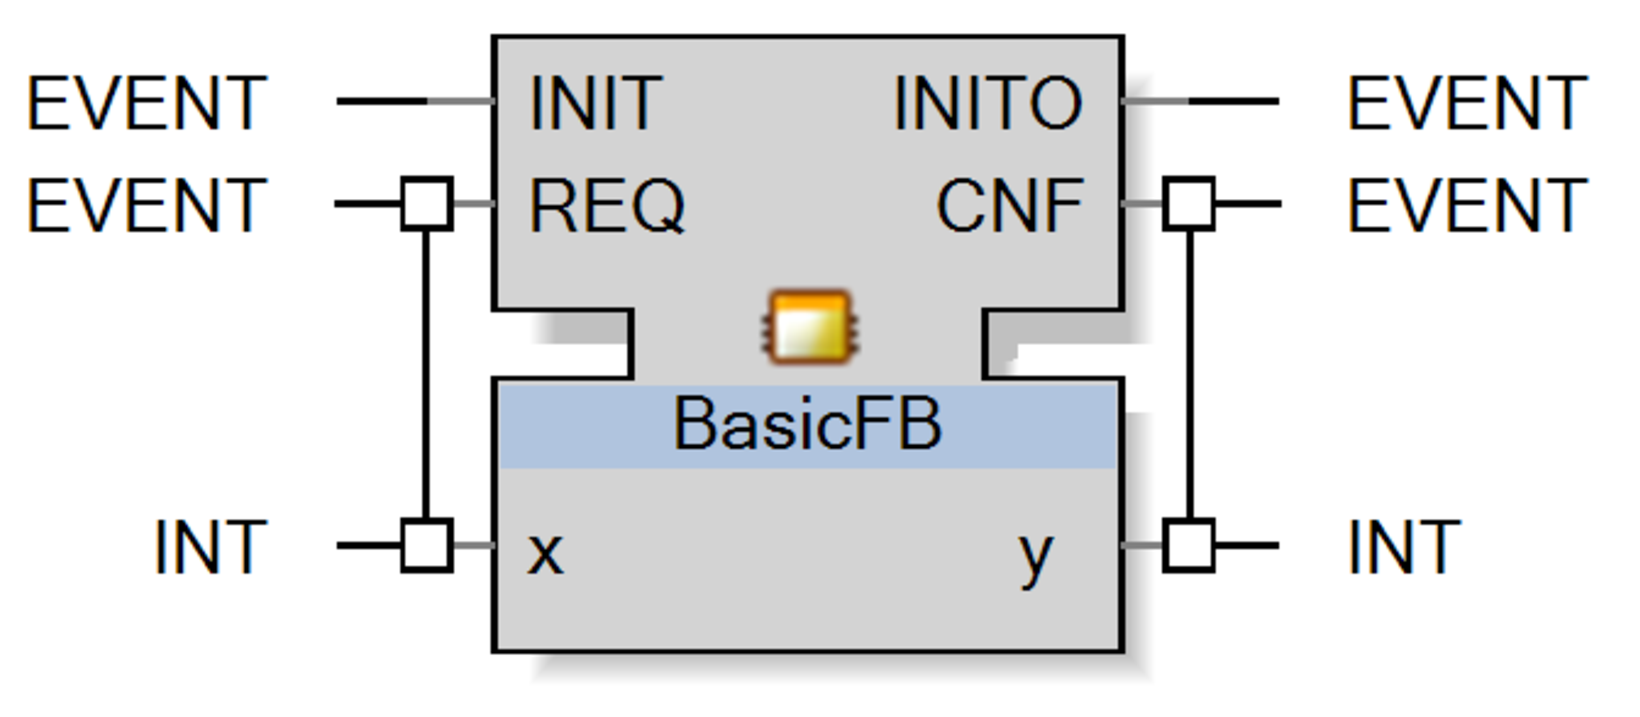
\includegraphics[width=2.5in]{pic/ecc-interface.eps}
    \caption{Пример интерфейса функционального блока}
    \label{fb-interface-example}
\end{figure*}

\begin{figure*}[t]
    \centering
    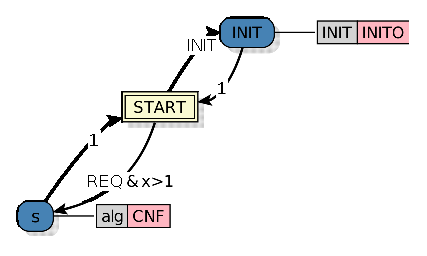
\includegraphics[width=2.5in]{pic/ecc-example.eps}
    \caption{Пример диаграммы управления исполнением функционального блока}
    \label{ecc-example}
\end{figure*}

\subsubsection{Темпоральные логики}

Темпоральная логика (\emph{temporal logic}) \cite{tl} --- это логика, учитывающая причинно-следственные связи в условиях времени.
Используется для описания последовательностей событий и их взаимосвязи по временной шкале.
Темпоральные логики часто применяются для выражения требований формальной верификации.

Язык темпоральной логики состоит из зависящих от проблемы
пропозициональных переменных, операторов булевой логики и набора темпоральных
операторов, таких как:

$G(f)$ означает, что $f$ должна выполняться во всех состояниях.

$X(f)$ означает, что $f$ должна выполняться в следующем состоянии.

$F(f)$ означает, что $f$ должна выполняться в каком-либо из будущих состояний.

Так как развитие описываемой системы может быть недетерминированно, то в каждом
состоянии могут существовать различные пути развитися системы. В рамках логики
деревьев вычислений (computation tree logic, CTL) допускается использование кванторов. Квантор $\forall$
требует, чтобы формула выполнялась на всех путях, исходящих из состояния, а
квантор $\exists$, чтобы существовал такой путь, на котором формула выполяется.
В рамках линейной темпоральной логики формула должна выполняться на всех путях.

\subsubsection{Сценарии исполнения}

Сценарий исполнения это последовательность четверок $\langle e, i, z, o
\rangle$, где $e : E$ -- входное событие, $i : \{0, 1\}^{|I|}$ -- вектор
значений входных переменных, $z : Z^*$ -- выходные события и $o :
\{0, 1\}^{|O|}$ -- вектор значений выходных переменных. Говорят, что диаграмма
управления исполнением удовлетворяет сценарию, если, будучи запущенной и
получая в качестве входных событий и переменных значения из сценария, она будет
выдавать соответствующие элементы четверок.

\subsubsection{Методы генерации конечных автоматов без учета темпоральных формул}

Задача генерации автоматов известна уже достаточно давно. Существуют различные методы
как точные так и эвристические для ее решения. Так например в \cite{ps, ask} использовались
генетические алгоритмы для построения автопилота для управления беспилотным
летательным аппаратом. В \cite{sat} предложено сведение задачи генерации детерминированных конечных автоматов
к задаче SAT. Позже, в работе \cite{csp} был предложен алгоритм, основанный на сведении к задаче
удовлетворения ограничениям (CSP).

\subsubsection{Постановка задачи}

Пусть $a$ -- набор формул линейной темпоральной логики, которым удовлетворяет
исходный блок, а $b$ -- набор сценариев, полученных при тестировании исходного
блока. Тогда нашей целью является нахождение такого автомата $c$, что
выполяются следующие условия.

1) $c$ удовлетворяет всем формулам из $a$.

2) $c$ удовлетворяет всем сценариям из $b$.

\subsection{Обзор используемых подходов}
\subsubsection{Верификация символьных моделей}

Система верифификации символьных моделей предназанчена для проверки систем с
конечным числом состояний на то, удовлетворяют ли они заданным темпоральным
свойствам. В языке SMV (simple model verification) переменные принадлежат конечным скалярным типам, а
программы состоят из параллельных операторов присвоения. Таким образом
программа может рассматриваться как система уравнений, а ее решением будет
следующее состояние модели. При этом запрещены множественное присвоение одной
переменной и циклические зависимости, что позволяет гарантировать, что решение
существует. Заметим так же, что решений может быть несколько, в этом случае мы
сталкивемся с недетерменированным поведением.

\subsubsection{Востановление логики функиональных блоков с использованием
метаэвристического алгоритма}

Так как наш подход основан на \cite{rec}, мы приведем краткий обзор метода синтеза
блоков из указанной работы. Этот метод основан на метаэвристической
оптимизации. Метаэвристический алгоритми используются для нахождения хороших
решений сложных проблем (например тех, для которых нахождение точного решения
вычислительно сложно) за разумное время.

Процесс поиска в \cite{rec} начинается с генерации случайных начальных кандидатов
(случайных диаграмм управления исполнением). Затем пространоство поиска,
которое является множеством все возможных диаграмм с фиксированным интерфейсом,
исследуется с помощью так называемых операторов мутации: процедур, которые
вносят некоторые изменения в структуру диаграмм. Например данные операторы
используются в \cite{rec}:

1) Выбрать случайный переход и изменить состояние, в которое он ведет.

2) Выбрать случайный переход и удалить его.

3) Выбрать случайное состояние и добавить переход в другое случайное состояние.

Каждый новый кандидат затем измеряется при помощи функции приспособленности:
она измеряет насколько хорошо решение удовлетворяет сценариям. Это происходит
следующим образом. Каждый сценарий обрабатывается по отдельности. На вход
диаграмме управления исполнением подаются входные значения из элементов
сценария, а выходные значения записываются. Затем значения, сгенерированные
диаграммой, сравниваются с соответствующими значениями сценария, использую
расстояние Левенштейна. Результаты нормализуются по отношению к длине сценария
и усредняются по всем сценариям. Функция приспособленности также измеряет
некоторые другие параметры: позицию первой ошибки (чем больше -- тем лучше) и
чесло переходов из одного состояния в другое в процессе исполнения (чем меньше
-- тем лучше).

Окончательная функция приспособленности выглядит следующим образом:
$$
F = c_1 F_{ed} + c_2 F_{fe} + c_3 F_{sc},
$$
где $F_{ed}$ основано на расстоянии Левенштейна, $F_{fe}$ на позиции первой
ошибки и $F_{sc}$ на числе изменеий состояний, а $c_1 - c_3$ -- константы.
Алгоритм оптимизации пытается максимизировать данную функцию.

\subsubsection{Верификации открытого и закрытого цикла}

Промышленные приложения обычно состоят из установки и контроллера. По стандарту
IEC 61499 оба представляются функциональными блоками. Здесь мы сконцентрируемся
на верификации контроллера.

Существуют два основных подхода к верификации систем установка-контроллер --
верификация открытого цикла и верификация закрытого цикла \cite{cl}. В верификации
открытого цикла контроллер верифицируется изолированно. И наоборот в
верификации закрытого цикла производится одновременная верификация контроллера
и модели установки. Второй подход более логичен чем первый, ведь мы
заинтересованны в поведении контроллера при работе с установкой. Более того, в
верификации открытого цикла мы сожем не иметь возможности верифицировать
некоторые верные утверждения т.к. ничего не ограничевает поведение установки.

Однако, у верификации закрытого цикла есть серьезная проблема -- нам нужна не
только формальная модель контроллера, но еще и формальная модель установки.
В некоторых случаях модель установки также может быть сгенерирована
автоматически \cite{dd}, но это может привести к очень большим моделям, которые будет
сложно верифицировать. Например даже при использовании техники абстрактной
установки \cite{dd}, верификация закрытого цикла для механического манипулятора заняла
294 секунды. Учитывая то, что в нашей работе нам придется верифицировать
большое количество кандидатов, такое большое время мы себе не можем позволить.

\subsection{Предлагаемый подход}

Для решения поставленной задачи а так же проблемы с верификацией закрытого
цикла, мы предлагаем следующий метод.  В его основе лежить параллельный
метод оптимизации, предложенный в \cite{rec}. Алгоритм расширяется с помощью новых
составляющих функции приспособленности и опреатора мутации. Верификация
кандидатов основана на заменителе модели установки, что сильно уменьшает время,
необходимое на верификацию. Мы испоьзуем NuSMV \cite{nusmv} для верификации SMV моделей
функциональных блоков.

\subsubsection{Верификация закрытого цикла с использованием заменителя модели
установки}

Подход, представленный в данной работе, лежит между верификациями открытого и
закрытого цикла. 

1) Модель контроллера. Создадим переменную $eccState : Y$ чтобы хранить
состояние контроллера. Для каждого входного и выходного события создадаим
булеву переменную, указывающую произошло событие или нет. Для каждой из
входных и выходных переменных создадим соответствующую ей переменную.

Изначально $eccState$ установлена в начальное состояние диаграммы. Затем, на
каждом шаге мы будем обновлять ее состояние исходя из ее текущего состояния,
входных событий и значений входных переменных. Выходные события и значения
выходных переменных вычисляются исходя из нового значения $eccState$. Выходные
действия могут заключаться генерации выходного события, установки значения
выходной переменной в $true$, установки значения выходной переменной в $false$
или сохранении текущего значения переменной.

2) Заменитель модели установки. Затем мы вручную создаем заменитель модели
установки и окружения и соединяем его с моделью контроллера. Все, что мы
требуем от заменителя, это то, он будет взаимодействовать с контроллером так,
как это делают реальные установка и окружение. Все другие детали избыточны. Это
значит, что заменитель модели может быть гораздо проще чем реальная модель
установки и окружения, что сильно ускоряет верификацию. Недостатком данного
подхода является то, что нам необходимо искать этот заменитель, что может быть
нетривиальной задачей.

\subsubsection{Функция приспособленности}

Получив спецификацию, состоящую из формул темпоральной логики, NuSMV проверяет
удовлетворяет ли данная SMV модель спецификации. Для каждой формулы он сообщает
либо то, что она удовлетворена, либо контрпример как доказательство того, что
она не удовлетворена.

Представим сперва новую компоненту функции приспособленности $F^{sat}_{smv}$ --
отношение числа удовлетворенных формул к общему из числу. Кроме того, будем
использовать в нашем алгоритме контрпримеры. Использование контрпримеров
вынуждает нас ограничиться линейной темпоральной логикой, исключив логику
деревьев вычислений. Это связано с тем, что для тех формул логики деревьев
вычислений, которые используют экзистенциальную квантификацию и не выполняются,
мы не можем привести контрпример т.к. попросту нет такого примера, который бы
доказывал, что некоторого пути не существует.

Мы так же будем использовать дополнительную компоненту $F^{ce}_{smv}$, которая
основана на длине наиболее длинного контрпримера $l_{max}$ для
неудовлетворенной формулы. Идея, которая стоит за этим, заключается в том, что
решения с более длинными контрпримерами, скорее всего лучше, чем решения с
короткими. Так как максимальной длины контрпримера не существует, мы
воспользуемся слудующей формулой.
$$
F^{ce}_{smv} = \begin{cases} 1, & \mbox{if} l_{max} = 0 \\
1 - \frac{1}{(1 + \frac{1}{10}l_{max})^{\frac{1}{10}}}, & \mbox{otherwise}
\end{cases}
$$
Значение $F^{ce}_{smv}$ равно еденице, когда $l_{max} = 0$ и стремится к
еденице, когда $l_{max} \rightarrow 1$, что нм как раз и нужно. Подводя итог,
наша функция приспособленности выглядит следующим образом:
$$
F = c_1 F_{ed} + c_2 F_{fr} + c_3 F_{sc} + c_4 F{sat}_{smv} + c_5 F^{ce}_{smv}.
$$

Проблема с использованием верификации в функции приспособленности заключается
в том, что даже несмотря на то, что мы не используем полную модель установки,
время, необходимое на верификацию, значительно больше, чем время, необходимое
для вычисления других компонент. Для решения данной проблемы мы предлагаем
следующий подход.

Вместо того чтобы вычислять компоненты основанные на верификации для каждого
решения, ма будем вычислять ее с некоторой вероятностью $p$, а с вероятностью
$1 - p$ использовать значения, вычисленные для предка решения. Конечно, это
может привести к потере некоторых хороших решений, однако такова цена.

Так же, если сумма остальных компонент выше некоторого порога, то мы всегда
производим верификацию. Это позволяет нам избежать потери решений близких к
оптимальному и гарантирует, что финальное решение действительно удовлетворяет
поставленной задаче.

\subsubsection{Оператор мутаций, использующий контрпримеры}

Как уже было отмечено ранее, в случае, если решение не удовлетворяет формуле,
NuSMV предоставляет контрпример. Контрпример можно рассматривать как сценарий
исполнения. В добавление к тому, что мы используем контрпримеры в функции
приспособленности, так же будем использовать их в специальном операторе
мутаций, схожий на представленный в \cite{et}. Особенность данного опреатора является то повышение вероятности
удаления или изменения переходов, входящих в контрпример.

Каждому переходу присваивается вес. Изначально вес каждого перехода равен
еденице. Затем мы будем исполнять контрпримеры и, каждый раз используя перход,
будем увеличивать его вес на величину $\lambda$. Затем воспользуемся методом
рулетки с вероятностями, пропорциональными весам, для того чтобы выбрать
переход и случайным образом изменить его.

\subsection{Экспериментальные результаты}

\begin{figure}[t]
    \centering
    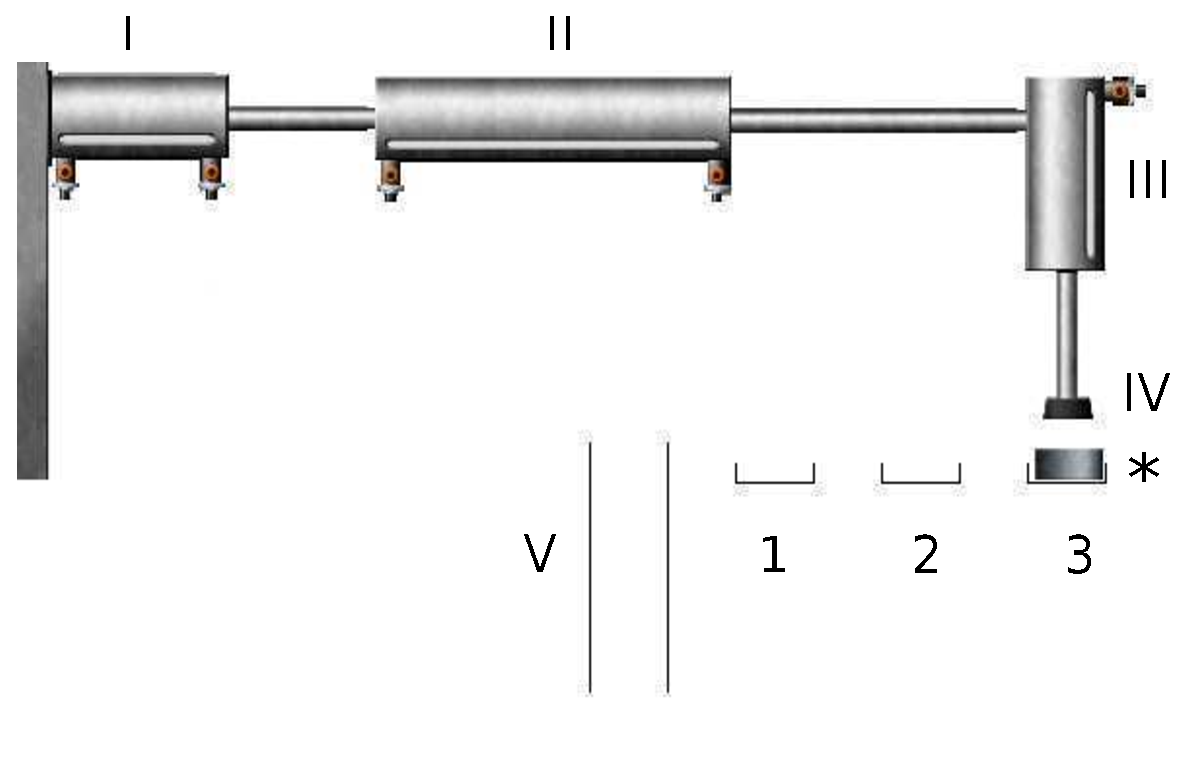
\includegraphics[width=3in]{pic/pnp.eps}
    \caption{Манипулятор подними-и-полжи с тремя цилиндрами}
    \label{pnp-system}
\end{figure}

Для тестирования данного подхода был использован манипулятор подними-и-положи \cite{pnp},
показанный на рисунке \ref{pnp-system}.
Он представляет собой механическую руку, три входных дорожки и одну выходную.
Рука состоит из двух горизонтальных цилиндра, которые могут выдвигаться и
вдвигаться. Четыре возможных комбинации позволяют позиционироваться над
каждой из четырех дорожек. 

В состав руки так же входит вертикальный цилиндр, который позволяет
перемещаться вверх и вниз всасывающему устройству, которое испоьзуется чтобы
поднимать детали с дорожек. У манипулятора есть сенсоры, которые определяют
положения цилиндров, находится ли что-то на входных дорожках, а так же
захвачено ли что-нибудь рукой. Задача манипулятора перемещать детали с входных
дорожек на выходную.

\subsubsection{Модель установки и среды}

Для каждой входной дорожки мы создадим две булевы переменных $p_i$ и $pp_i$.
Значения $p_i$ мы не ограничивает, таким образом они моделирую
недетерменированное появление деталей, а значения $pp_i$ определяются
следующим образом. Если в данный момент рука поднимает деталь с $i$-ой
дорожки, то $pp_i := false$, если $pp_i = true$, то ее значение сохраняется
иначе $pp_i := p_i$. Таким образом мы моделируем поведение, когда деталь
может появиться на дорожке в произвольный момент времени, но появившись
остается там до тех пор, пока не будет захвачена рукой.

Всасывающее устройство моделируется единственной переменной, указывающей
включено устройство или выключено. Если контроллер подает команду включить
или выключить устройство, мы изменяем переменную соответствующим образом,
иначе оставляем ее нетронутой.

Так как цилиндры двигаются не мгновенно, для каждого из них создадим переменную
$cs_i : \{cst_j | j = 0 .. 3 \}$, хранащую состояние цилиндра. Будем изменять
эти переменные в соответствии с командами контроллера. В свою очередь сенсоры
будут использовать эти переменные для определения положения цилинлра.

Последнее, что нам осталось сделть это задать работу индикатора того держит
ли рука что-нибудь или нет. Для этого создадим переменную $vac$. Алгоритм
вычисления ее значения прост. Если всасывющее устройство выключено, то
$vac := false$, если всасывющее устройство расположено наж дорожкой с деталью,
вертикальный цилиндр выдвинут и устройство включено, то $vac := true$, иначе
ее значение сохраняется.

Общая схема работы модели такова. На каждом шаге мы генерируем входное событие
и просим перещитать свое состояние. Это происходит в соответствии с диаграмой
управелия исполнением, текущим состоянием модели и значениями входных
переменных. Затем мы перещитываем состояние окружения исходя из его текущего
состояния, значений выходных переменных контроллера и вышеуказанных правил.

\subsubsection{Эксперименты}

Наши эксперименты преследовали несколько целей. Во-первых, проверить и
продемонстрировать практическую применимость данного подхода, а, во-вторых,
проверить, что исползование длины контрпримеров в функции приспособленности
приводит к улучшению работы алгоритма.

Мы использовали один сценарий, соответствующий обработке одной детали на
первой дорожке. Длина этого сценария 2339. Так же были использованы
следующие три темпоральных свойства:
\begin{enumerate}
    \item $G(\lnot (c1Extend \wedge c1Retract))$~-- свойство безопасности, гласящее, что
первый цилиндр не должен получать команд на выдвижение и вдвижение одновременно;
    \item $G(\lnot (c2Extend \wedge c2Retract))$~-- аналогичное свойство для второго цилиндра;
    \item $G(pp1 \rightarrow F(vp1))$~-- функциональное свойство, гласящее, что, если деталь
появилась на дорожке, то когда-нибудь она будет обработана.
\end{enumerate}

Алгоритм был реализован на языке Java и доступен по адресу https://github.com/V1489Cygni/spec2fb.
Мы использовали NuSMV 2.5.4 для верификации
темпоральных свойств и запускали его с параметрами по умолчанию. Все эксперименты
проводились на машине с 64-ядерным AMD Opteron\texttrademark 6378 @ 2.4 GHz процессором.
Использовались 16 ядер и 32 гигабайта оперативной памяти.

Сперва мы использовали только сценарий в качестве входных данных и провели 50 запусков.
Затем провели запуски, использовав темпоральные свойства, но не используя длину
контрпримеров в функции приспособленности. И в конце были проведены запуски полной
системы. Результаты приведены в таблице \ref{results-table}.

Во-первых, отметим, что все сгенерированные решения удовлетворяли первым двум
темпоральным свойствам. Это было ожидаемо так как это свойства безопасности ---
они описывают что система делать не должна. Они могут быть удовлетворены даже
если система не делает ничего.

Во-вторых, ни одно из сгенерированных без темпоральных формул решений не удовлетворило
третьей формуле. Это подтверждает, что весьма маловероятно, что случайно будет
сгенерировано решение, удовлетворяющее функциональным темпоральным свойствам.

В-третьих, использование темпоральных верификации в функции приспособленности привело
к генерации решений, которые удовлетворяли всем формулам. Так же очевидно, что использование
верификации привело к значительному увеличению времени работы алгоритма. В свою очередь,
использование длины контрпримеров в функции приспособленности привело к ускорению на 30\%.

После генерации все решения было проверены в системе FBDK\footnote{\url{http://www.holobloc.com/doc/fbdk}}.
Все решения, сгенерированные с учетом темпоральных свойств успешно обрабатывали дорожку несколько раз,
в то время как решения, сгенерированные только по сценарию, не обрабатывали ее более одного раза.

\subsection{Заключение}

В данной работе был представлен подход для генерации простых функциональных блоков по
сценариям и темпоральным свойствам. Верификация была встроена в функцию приспособленности и
опреатор мутации. Верификация проводится по способу закрытого циклас использованием
вручную написанной модели среды и установки. Эта модель отображает внешнее поведение
установки и гораздо проще чем полная модель.

Представленный подход достиг успеха, сгенерировав диаграммы управления состоянием для
описанного манипулятора, которые выполняли поставленную задачу --- перемещать детали
с входной дорожки на выходную. При помощи добавления верификации мы смогли гарантировать,
что такое поведение будет наблюдаться необходимое число раз, что не наблюдается в
результатах полученным лишь по сценариям.

По резултатам данной работы была написана и принята на конференцию статья \cite{this}.

\pagebreak

\begin{thebibliography}{99}
\addcontentsline{toc}{subsection}{Литература}

\bibitem{iec}
V. Vyatkin, “IEC 61499 as Enabler of Distributed and Intelligent
Automation: State-of-the-Art Review,” IEEE Transactions on Industrial
Informatics, vol. 7, no. 4, pp. 768–781, Nov 2011.

\bibitem{rec}
D. Chivilkhin, A. Shalyto, S. Patil, and V. Vyatkin, “Reconstruction of
function block logic using metaheuristic algorithm: Initial explorations,”
in Proceedings of IEEE International Conference on Industrial Informat-
ics, 2015, pp. 1239–1242.

\bibitem{ea}
T. Back, D. B. Fogel, and Z. Michalewicz, Eds., Handbook of Evolu-
tionary Computation. Bristol, UK: IOP Publishing Ltd., 1997.

\bibitem{cl}
V. Vyatkin, H.-M. Hanisch, C. Pang, and C.-H. Yang, “Closed-loop
modeling in future automation system engineering and validation,”
Systems, Man, and Cybernetics, Part C: Applications and Reviews, IEEE
Transactions on, vol. 39, no. 1, pp. 17–28, Jan 2009.

\bibitem{dd}
S. Patil, D. Drozdov, V. Dubinin, and V. Vyatkin, Technological
Innovation for Cloud-Based Engineering Systems: 6th IFIP WG
5.5/SOCOLNET Doctoral Conference on Computing, Electrical and
Industrial Systems, DoCEIS 2015, Costa de Caparica, Portugal, April
13-15, 2015, Proceedings. Cham: Springer International Publishing,
2015, ch. Cloud-Based Framework for Practical Model-Checking of
Industrial Automation Applications, pp. 73–81. [Online]. Available:
http://dx.doi.org/10.1007/978-3-319-16766-4 8

\bibitem{nusmv}
A. Cimatti, E. Clarke, E. Giunchiglia, F. Giunchiglia, M. Pistore,
M. Roveri, R. Sebastiani, and A. Tacchella, “NuSMV Version 2: An
OpenSource Tool for Symbolic Model Checking,” in Proc. International
Conference on Computer-Aided Verification (CAV 2002), ser. LNCS, vol.
2404. Copenhagen, Denmark: Springer, 2002.

\bibitem{pnp}
S. Patil, V. Vyatkin, and M. Sorouri, “Formal verification of Intelligent
Mechatronic Systems with decentralized control logic,” in Proceedings
of the 17th IEEE Conference on Emerging Technologies Factory Au-
tomation, 2012, pp. 1–7.

\bibitem{et}
F. Tsarev and K. Egorov, “Finite state machine induction using genetic
algorithm based on testing and model checking,” in Proceedings of
the 13th Annual Conference Companion on Genetic and Evolutionary
Computation, ser. GECCO ’11. New York, NY, USA: ACM, 2011, pp.
759–762.

\bibitem{tl}
A. Pnueli. The temporal logic of programs.
In Foundations of Computer Science, 1977., 18th Annual Symposium on, pages 46–57, Oct 1977.

\bibitem{this}
Chivilikhin D., Ivanov I., Shalyto A., Vyatkin V. Reconstruction of Function Block
Controllers Based on Test Scenarios and Verification / To appear in Proceedings of
the 14th IEEE International Conference on Industrial Informatics, 2016.

\bibitem{ps}
Поликарпова Н. И., Точилин В. Н., Шалыто А. А.
Метод сокращенных таблиц для генерации автоматов с большим числом входных
переменных на основе генетического программирования // Известия РАН.
Теория и системы управления. — 2010. — № 2. — С. 100—117.

\bibitem{ask}
Genetic algorithm for induction of finite automata with continuous and
discrete output actions / A. Alexandrov, A. Sergushichev, S. Kazakov,
F. Tsarev // Proceedings of the 13th annual conference companion on
Genetic and evolutionary computation. — New York, NY, USA : ACM,
2011. — P. 775–778.

\bibitem{sat}
Heule M., Verwer S. Exact DFA Identification Using SAT Solvers // Proceedings
of the 10th International Colloquium Conference on Grammatical
Inference: Theoretical Results and Applications. — Berlin, Heidelberg
: Springer-Verlag, 2010. — P. 66–79.

\bibitem{csp}
Chivilikhin D., Ulyantsev V., Shalyto A. Combining Exact and Metaheuristic
Techniques for Learning Extended Finite-State Machines from
Test Scenarios and Temporal Properties // Proceedings of the 13th International
Conference on Machine Learning and Applications. — IEEE
Computer Society, 2014. — P. 350–355.

\end{thebibliography}

\end{document}
